\documentclass[10pt]{article}
\usepackage{epsf}
\usepackage{amsmath}
\usepackage{amssymb}
\usepackage{palatino}
\usepackage[pdftex]{graphics}
\usepackage{fancyhdr}
\usepackage{epsfig}
\usepackage{multirow}
\usepackage{multicol}
\usepackage{cancel}
\usepackage{hyperref}
\usepackage{longtable}
\usepackage{ulem}
\usepackage[yyyymmdd]{datetime}
\renewcommand{\dateseparator}{-}
\usepackage{listings}

\parindent 0in
\parskip 1ex
\oddsidemargin  0in
\evensidemargin 0in
\textheight 8.5in
\textwidth 6.5in
\topmargin -0.25in

\pagestyle{fancy}
\lhead{\textbf{\leftheader}}
\rhead{\textbf{\rightheader}}
\lfoot{Compiled: \today\ \currenttime}
\cfoot{}
\rfoot{\thepage}

\newcommand{\leftheader}{BME290L: MedTech Prototyping Skills}
\newcommand{\rightheader}{Palmeri (Spring 2023)}

\begin{document}

\title{Lab 06: PCB Layout} 
\author{MedTech Prototyping Skills (BME290L)}
\maketitle

\section{PCB Layout}
You will be laying out a PCB of your circuit using the following guidelines:
\begin{itemize}
    \item Be sure to update the PCB metadata in \texttt{Page Settings} (these are \textbf{not} inherited from the schematic).
    \item Be sure to setup your \textbf{Design Rules} as follows:
    \begin{itemize}
        \item Signal trace widths should be $\geq$ 0.52 mm
        \item Power traces widths should be $\geq$ 1.0 mm
        \item Clearance on all traces should be $\geq$ 0.85 mm
        \item All drill hole diameters (including vias) should be $>$ 0.8mm
    \end{itemize}
    \item Your PCB can be two-sided.
    \item Remember that the traces for THT components should be on the opposite side of the component body.
    \item Utilize large \texttt{GND} pours.
    \item Make sure that your \textbf{Design Rules Checker} passes 100\%.
    \item Add your Name to one Cu layer of the board
    \item \textbf{Design Challenge}
    \begin{itemize}
        \item Make the board as small as possible, maintaining 4 mounting holes.
        \item Too small will make populating the board with components
            difficult.  Remember, small doesn't win over function.
        \item Be sure to place your testing points in convenient locations to
            verify function while populating the board with components and to
            do downstream functional analysis.
    \end{itemize}
\end{itemize}

\section{Generating PCB Layer PDFs}

To generate a PDF of your front and back layers, use the \texttt{File -> Plot} command with the following options:

\centerline{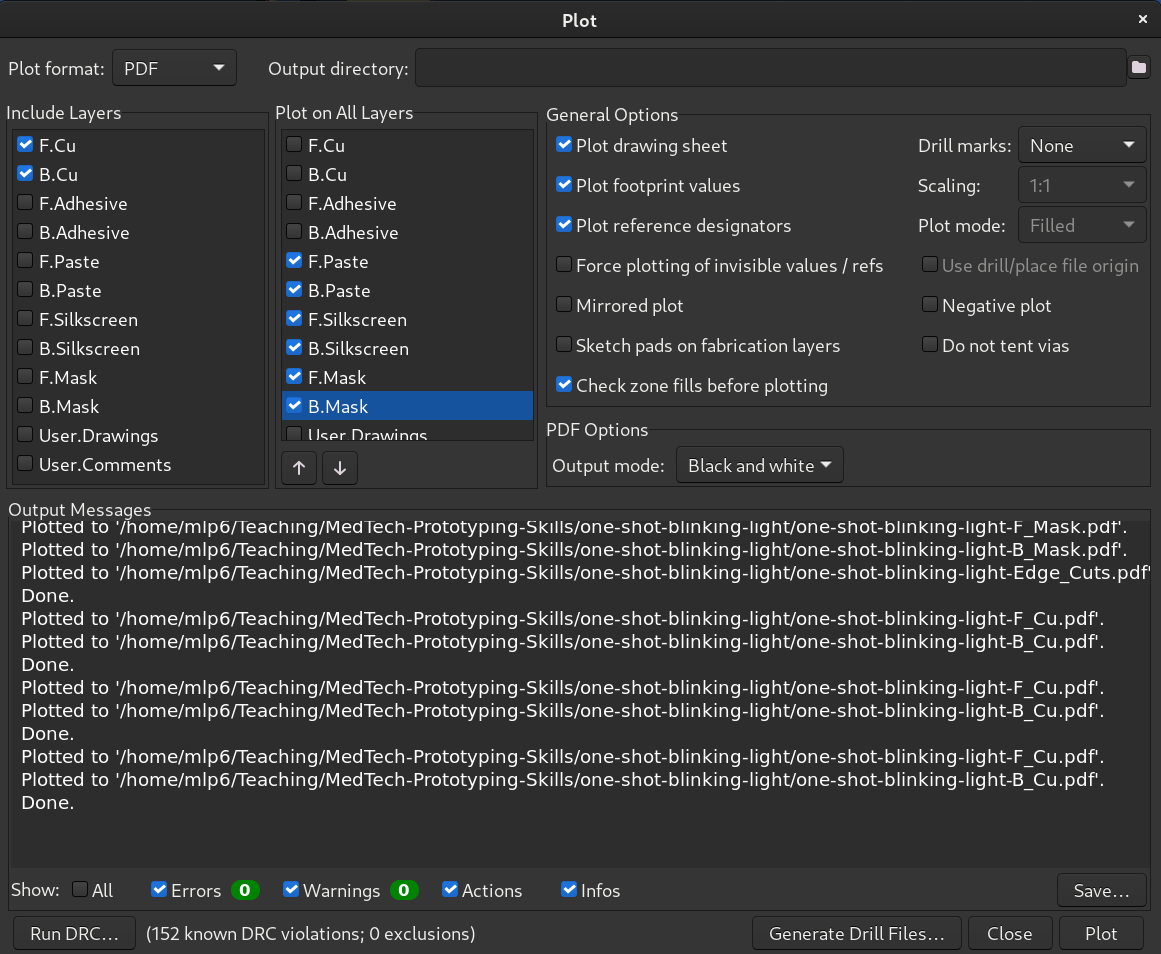
\includegraphics[width=1.0\textwidth]{pcb_pdf_plot.png}}

This will generate 2 PDF files (\texttt{\*-[F,B]\_Cu.pdf}) with the relevant mask
and silkscreen layers superimposed. 

An example of a rendered (incomplete) front and back layers:

\centerline{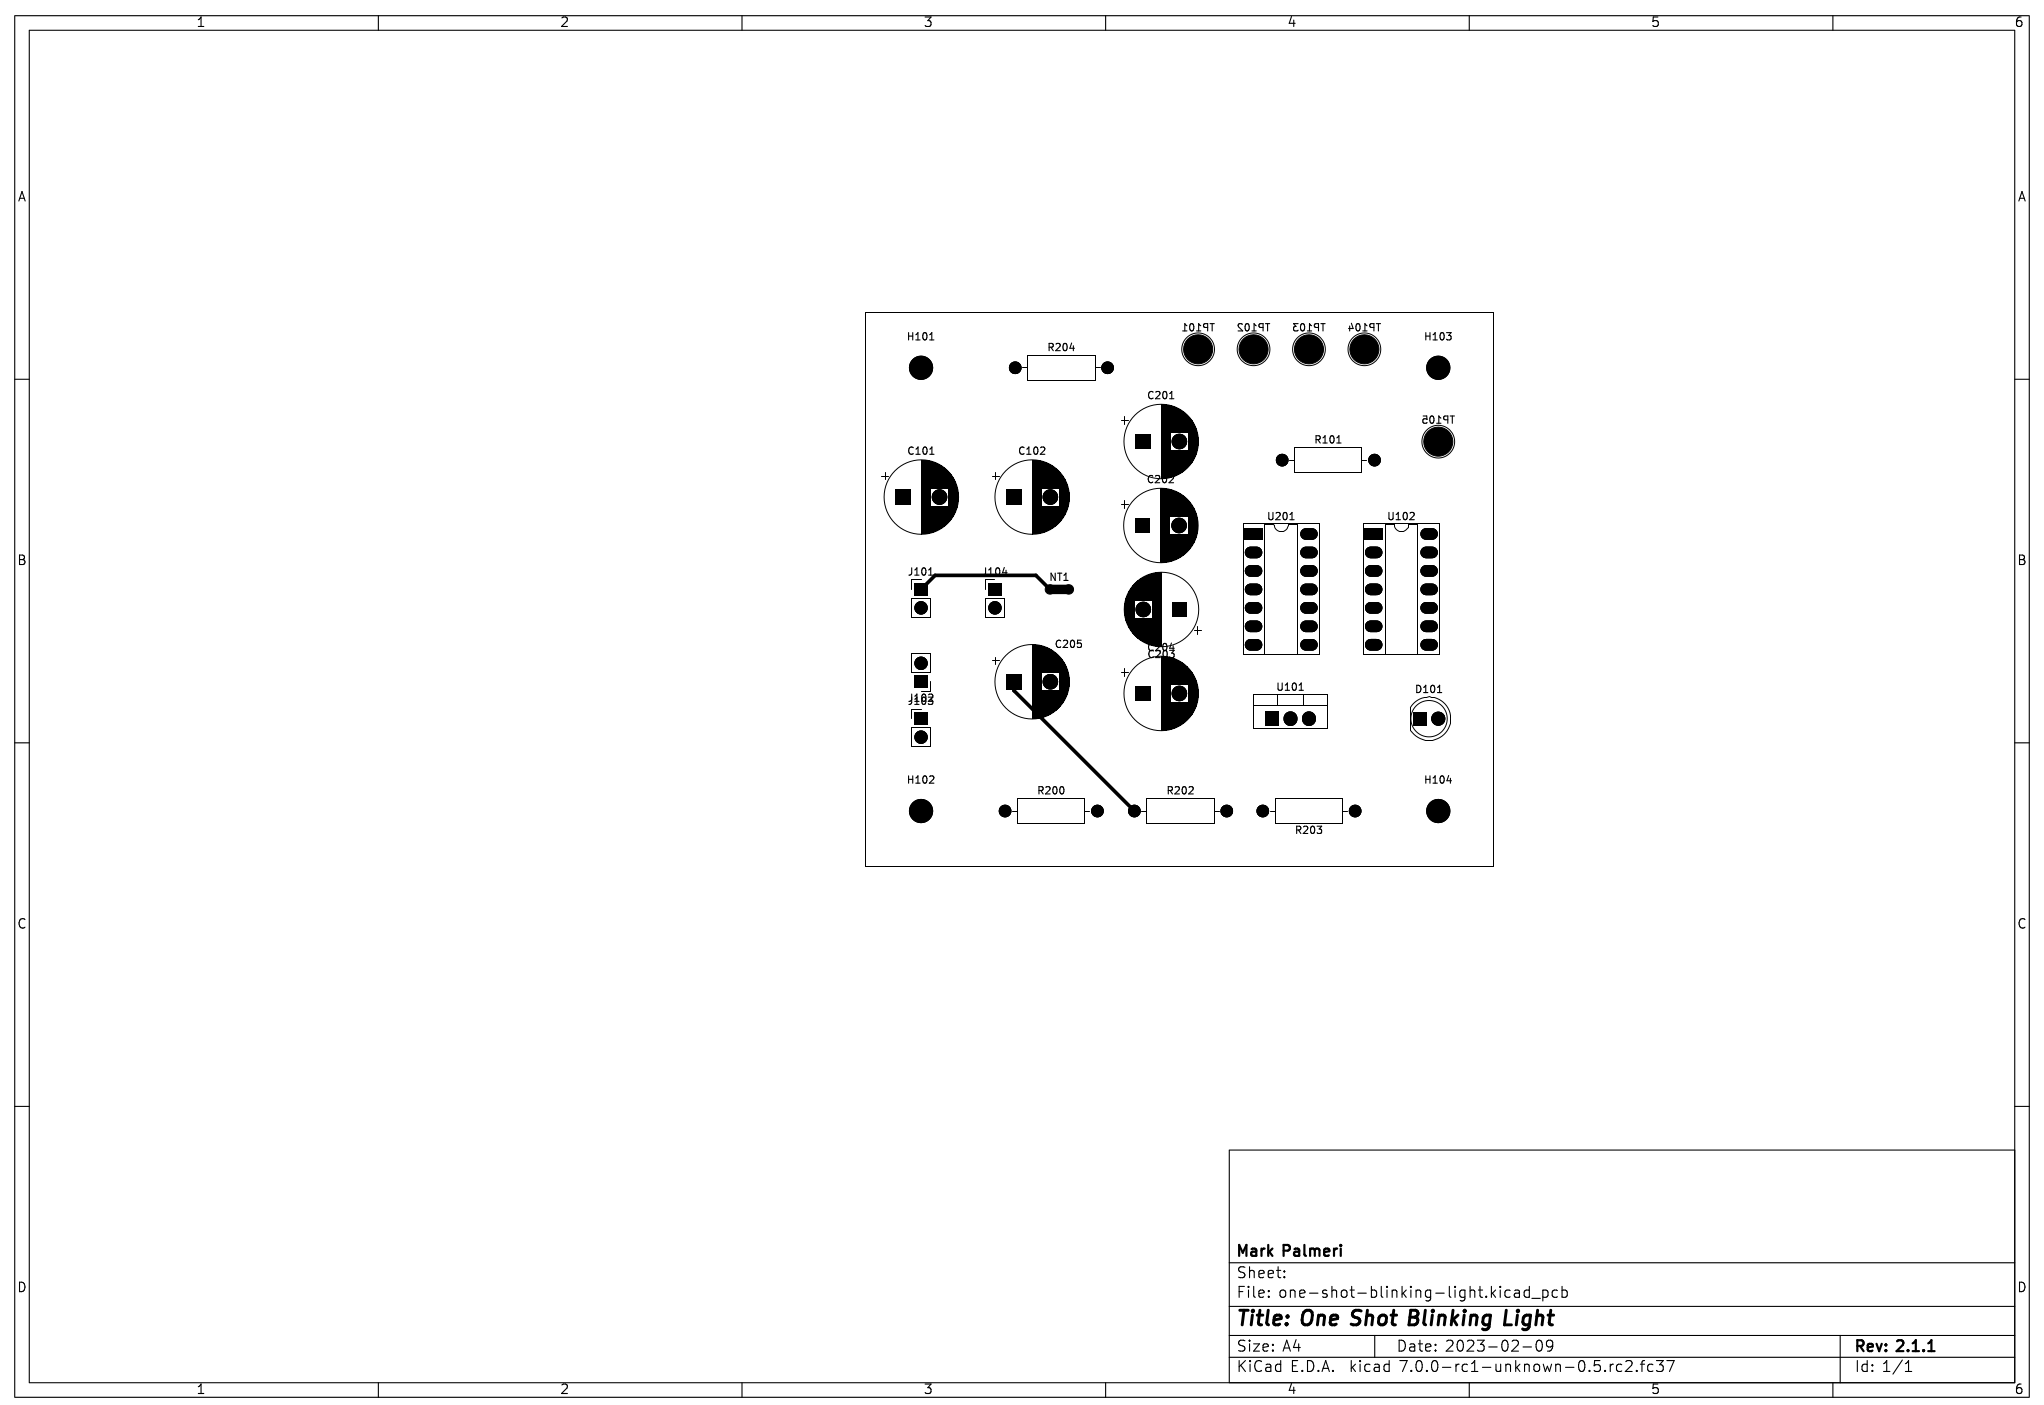
\includegraphics[width=0.5\textwidth]{example_F_Cu.png}}
\centerline{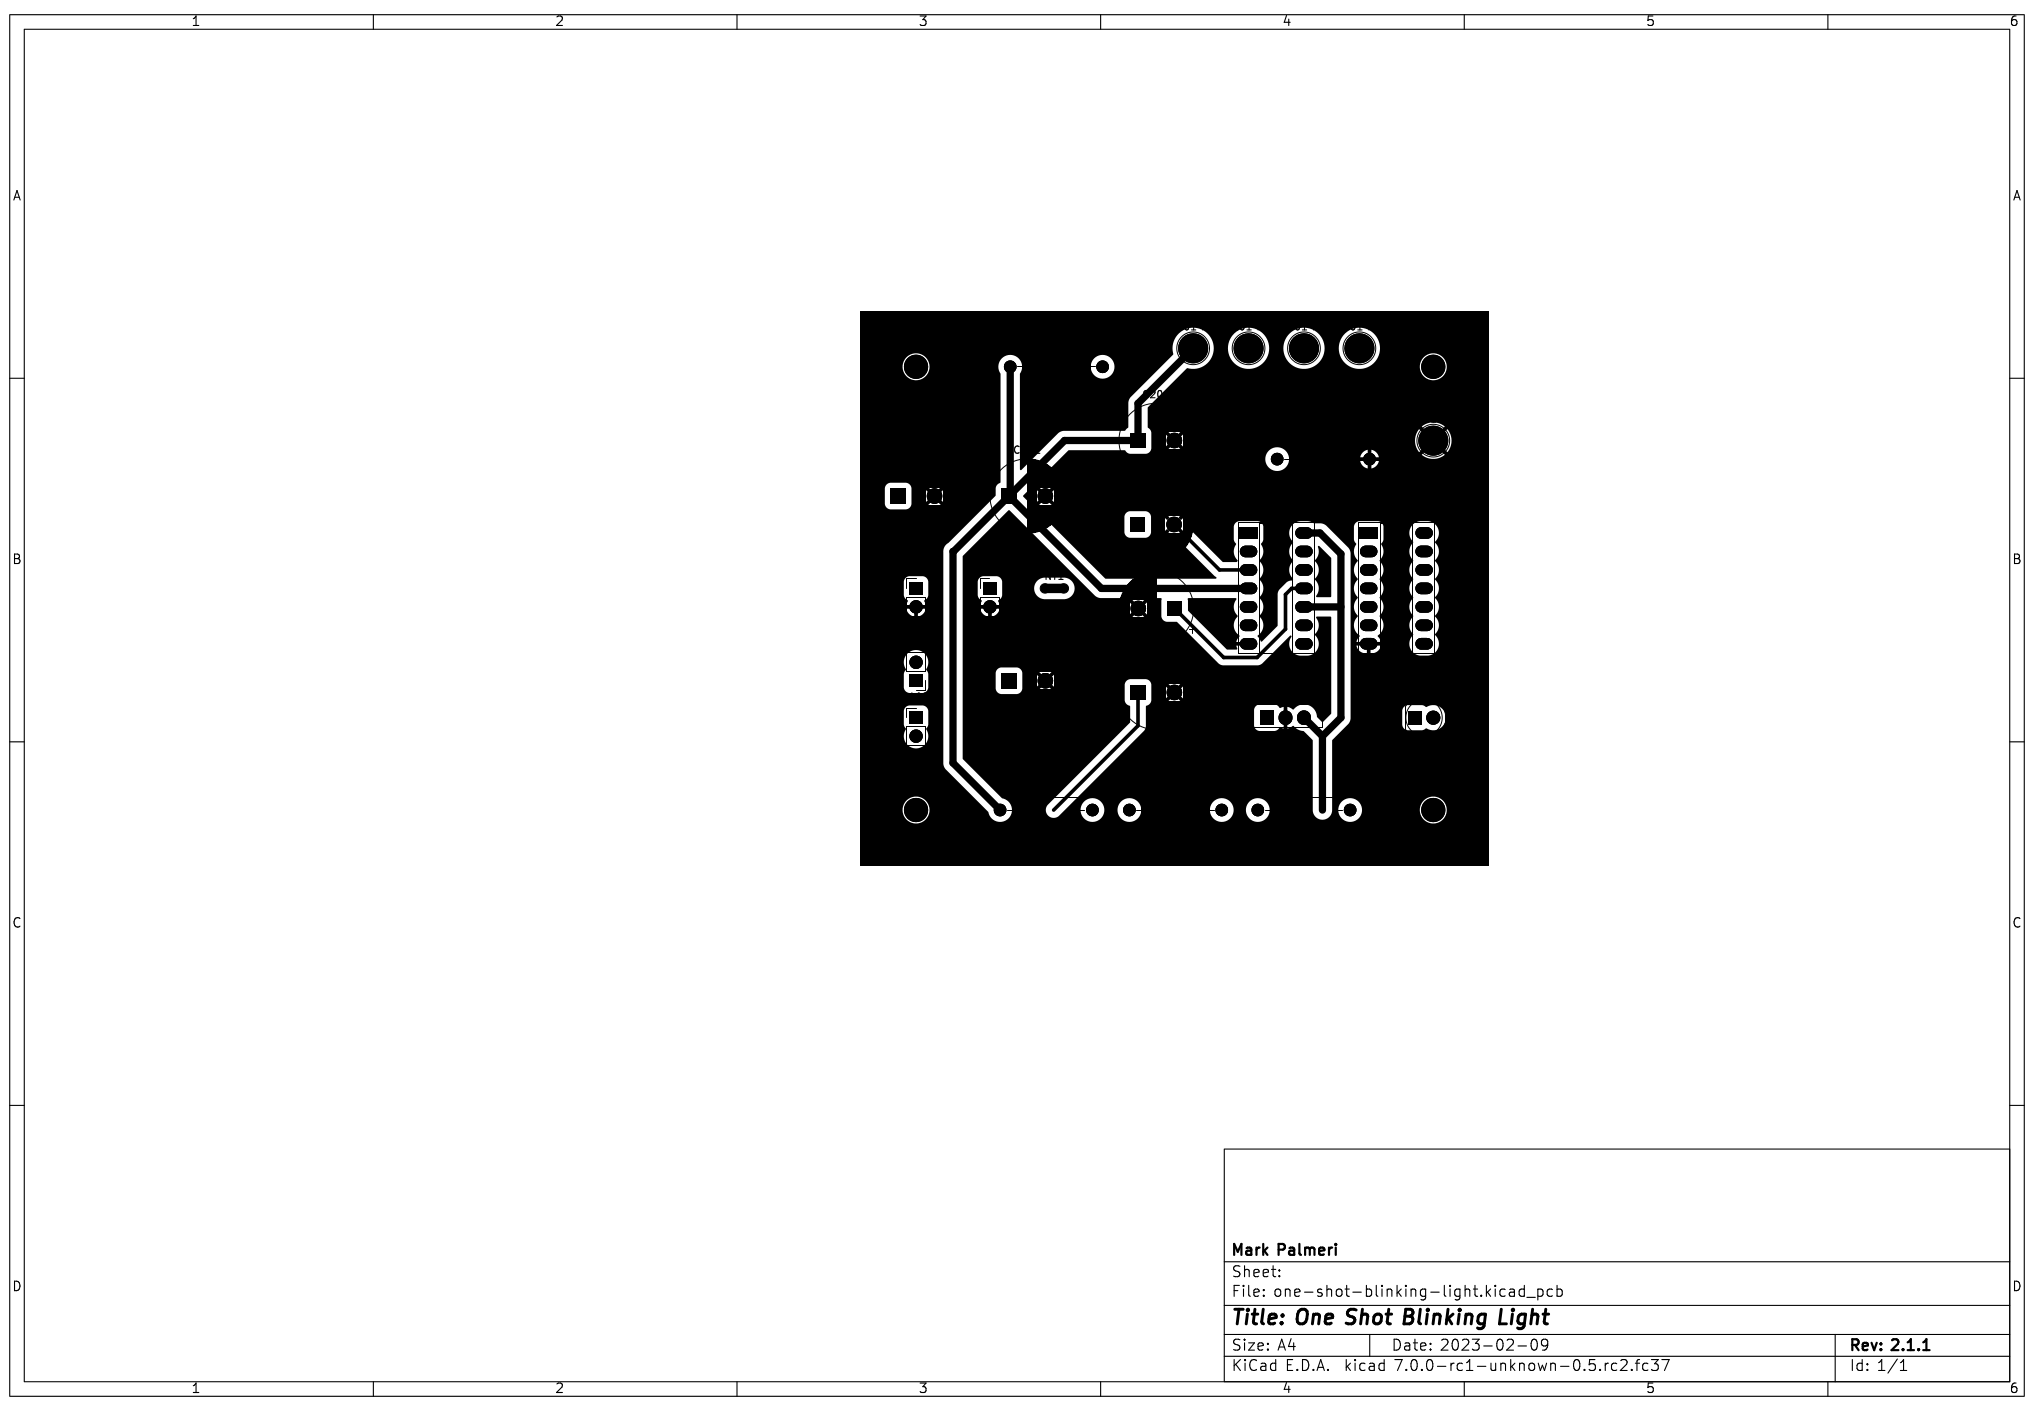
\includegraphics[width=0.5\textwidth]{example_B_Cu.png}}

\section{What to Submit}
\begin{enumerate}
    \item A single PDF to Gradescope containing:
    \begin{itemize}
        \item View of front layer (make sure all zones filled)
        \item View of back layer (make sure all zones filled)
        \item Screenshot of 3D view
        \item Export of your Design Rules Checker report
            (\texttt{DRC.rpt}).\footnote{This report is an ASCII text file that
            can be convered to a PDF.}
    \end{itemize}
    \item Upload a zip archive of your entire project to your \textbf{Drop Box}
        on Sakai.  Please use the following naming scheme for your zip file:
        \texttt{LastNameFirstName\_v3.X.X.zip}.  
        
        For example: \texttt{PalmeriMark\_v3.0.0.zip}
\end{enumerate}

\end{document}
